\documentclass[draft=True]{thesis}
\usepackage{graphicx, slashed, siunitx}
\usepackage[utf8]{inputenc}
\usepackage{xr-hyper}
\documentclass[a4paper,10pt,draft]{thesis}
\usepackage{physics,amsmath, amsfonts, siunitx, amssymb, graphicx, slashed,subcaption}
\usepackage[utf8]{inputenc}
\usepackage[margin=1in]{geometry}
\usepackage[hidelinks]{hyperref}
\usepackage{xr-hyper}
\newcommand{\n}[1]{\nu_{#1}}
\newcommand{\na}{\nu_\alpha}
\newcommand{\nb}{\nu_\beta}
\newcommand{\ana}{\bar{\nu}_\alpha}
\newcommand{\an}[1]{\bar{\nu}_{\text{#1}}}
\newcommand{\anb}{\bar{\nu}_\beta}
\renewcommand{\a}{\alpha}
\renewcommand{\b}{\beta}
\newcommand{\ab}{\alpha\beta}


\renewcommand{\ne}{\nu_e}
\newcommand{\nm}{\nu_\mu}
\newcommand{\nt}{\nu_\tau}
\newcommand{\ns}{\nu_s}

\newcommand{\ane}{\bar{\nu}_e}
\newcommand{\anm}{\bar{\nu}_\mu}
\newcommand{\ant}{\bar{\nu}_\tau}
\newcommand{\ans}{\bar{\nu}_s}

\newcommand{\nee}{\nu_e \to \nu_e}
\newcommand{\nem}{\nu_e \to \nu_\mu}
\newcommand{\net}{\nu_e \to \nu_\tau}
\newcommand{\nes}{\nu_e \to \nu_s}

\newcommand{\nme}{\nu_\mu \to \nu_e}
\newcommand{\nmm}{\nu_\mu \to \nu_\mu}
\newcommand{\nmt}{\nu_\mu \to \nu_\tau}
\newcommand{\nms}{\nu_\mu \to \nu_s}



\newcommand{\Pee}{P_{e  e}}
\newcommand{\Pem}{P_{e  \mu}}
\newcommand{\Pet}{P_{e  \tau}}
\newcommand{\Pes}{P_{e  s}}

\newcommand{\Pme}{P_{\mu  e}}
\newcommand{\Pmm}{P_{\mu\mu}}
\newcommand{\Pmt}{P_{\mu  \tau}}
\newcommand{\Pms}{P_{\mu  s}}


\newcommand{\Pte}{P_{P_{\tau e}}}
\newcommand{\Ptm}{P_{\tau  \mu}}
\newcommand{\Ptt}{P_{\tau  \tau}}
\newcommand{\Pts}{P_{\mu  s}}

\newcommand{\Paeae}{P_{\bar{e}  \bar{e}}}
\newcommand{\Paeam}{P_{\bar{e}  \bar{\mu}}}
\newcommand{\Paeat}{P_{\bar{e}  \bar{\tau}}}
\newcommand{\Paeas}{P_{\bar{e}  \bar{s}}}

\newcommand{\Pamae}{P_{\bar{\mu}  \bar{e}}}
\newcommand{\Pamam}{P_{\bar{\mu}  \bar{\mu}}}
\newcommand{\Pamat}{P_{\bar{\mu}  \bar{\tau}}}
\newcommand{\Pamas}{P_{\bar{\mu}  \bar{s}}}


\newcommand{\Patae}{P_{\bar{\tau}  \bar{e}}}
\newcommand{\Patam}{P_{\bar{\tau}  \bar{\mu}}}
\newcommand{\Patat}{P_{\bar{\tau}  \bar{\tau}}}
\newcommand{\Patas}{P_{\bar{\mu}  \bar{s}}}

\renewcommand{\th}[1][]{%
  \theta\ifx\\#1\\\else_\text{#1}\fi
}
\newcommand{\thm}[1][]{%
  \theta^\text{M}\ifx\\#1\\\else_\text{#1}\fi
}
\renewcommand{\t}[1]{\text{{#1}}}
\newcommand{\avg}[1]{\left\langle {#1} \right \rangle}
\newcommand*{\dm}[1][]{%
  \Delta m^2\ifx\\#1\\\else_\text{#1}\fi
}
\newcommand{\zreco}{\cos{(\theta_z^{reco})}}
\newcommand{\ztrue}{\cos{(\theta_z^{true})}}
\newcommand{\z}{\cos{(\theta_z)}}
\newcommand{\Ereco}{E^{reco}}
\newcommand{\Etrue}{E^{true}}
\newcommand{\Aeff}{A^\text{eff}}
\newcommand{\emm}{\epsilon_{\mu\mu}}
\newcommand{\emt}{\epsilon_{\mu\tau}}
\newcommand{\eet}{\epsilon_{e\tau}}
\newcommand{\eem}{\epsilon_{e\mu}}
\newcommand{\ett}{\epsilon_{\tau\tau}}
\newcommand{\ep}{\epsilon^\prime}

\begin{document}

\section{Atmospheric neutrino flux}
The flux comes from \cite{hondapaper} %TODO: talk about flux
The flux data is binned in $\ztrue$ and has the following form

\begin{tabular}{lrrrrrrr}
    %\toprule
           $\Etrue$ [\si{\GeV}] &        $\phi_\mu$ &     $\phi_\bar{\mu}$ &        $\phi_e$ &     $\phi_{\bar{e}}$ &  $\ztrue_{min}$ &  $\ztrue_{max}$\\
    %\midrule
       27825.594022 &  6.060061e-12 &  3.167883e-12 &  1.558607e-13 &  1.038747e-13 &   -0.2 &   -0.1 \\
      247707.635599 &  5.940855e-16 &  2.923931e-16 &  1.364937e-17 &  8.115912e-18 &   -0.7 &   -0.6 \\
         22.387000 &  3.328100e-02 &  2.781700e-02 &  9.565800e-03 &  7.149400e-03 &   -0.3 &   -0.2 \\
      432876.128108 &  5.185841e-17 &  2.320702e-17 &  1.456761e-18 &  9.828299e-19 &   -1.1 &   -1.0 \\
       64280.731173 &  1.582403e-13 &  8.095293e-14 &  3.480179e-15 &  2.211758e-15 &   -0.4 &   -0.3 \\
    %\bottomrule
\end{tabular}

The fluxes are averaged over azimuthal direction and over solar minimun/maximum. The units of the fluxes are given as \si{\GeV^-1 \metre^-2 \second^-1 \steradian^-1}. 
We note that the fluxes for $\nt$ and $\nu_\bar{\tau}$ are missing. This is due to the rapid decay (and hence, low flux) of the $\tau$. Thus, we never have to use probabilities on the form 
$P_{\tau \beta}$, since we have no incoming $\nu_\tau$. 

After interpolating this data, we can plot the raw data together with its interpolated values.
%TODO: flux interpolated figure.


\section{Event reconstruction}
After an event has occurred, the IceCube algorithms process the data coming from the detector to \emph{reconstruct} the event. This means that, given the parameters recorded by the detector, what are their "true" values?
We are interested in two variables: the energy and the direction. Each event is tagged with a probable energy and zenith angle, called the recostructed parameters $\Ereco$ and $\zreco$, which are the parameters according to the DOMs.
The collaboration then uses numerous sophisticated methods to backtrack the reconstructed parameters to the true parameters. So a charged lepton hits the DOMs, and we ultimately end up with the associated neutrino's true and reconstructed energy and zenith angle. The reconstructed parameters are what we are using to analyze the data (because this is what the detector actually sees), while the true parameters are used in the determination of that neutrino's "actual" flux and cross-section (because this is what nature sees).

How do we then translate between the reconstructed and true parameters? In this work, we are using two different methods, which are based on the form of data available to us. 

\section{IceCube event count}\label{ch:ICmethod}
%TODO: show IC MC data

As the neutrinos have propagated the Earth, they arrive at the South Pole, where they interact in the ice to form their charged leptons. We now are interested in the effective area, i.e.~the detector area that the lepton "sees".
The effective area, $\Aeff$, depends on several parameters, some of them being detector physical volume, $\Etrue$,$\ztrue$ and the neutrino cross-section. Fortunately, the binned $\Aeff$ is provided to us by the ICeCube collaboration~\cite{ICaeff}.
The data file has the following form

\begin{tabular}{lrrrrr}
    %\toprule
    $\Etrue_{min}$ [\si{\GeV}] &     $\Etrue_{max}$ [\si{\GeV}]&   $\ztrue_{min}$ &   $\ztrue_{max}$ &     $\Aeff$ [\si{\metre\squared}] \\
    %\midrule
         251.2 &      316.2 &  -0.92 &  -0.91 &   0.0174 \\
      794300.0 &  1000000.0 &  -0.80 &  -0.79 &  69.3600 \\
        3981.0 &     5012.0 &  -0.78 &  -0.77 &   3.1490 \\
        1585.0 &     1995.0 &  -0.07 &  -0.06 &   0.4659 \\
        398.1 &      501.2 &  -0.73 &  -0.72 &   0.0555 \\
    %\bottomrule
    \end{tabular}
Here, $\Aeff$ has been averaged over $\Aeff_\mu$ and $\Aeff_\bar{\mu}$. Thus, it is not flavor dependent.
Just as with the fluxes, we interpolate this in $\Etrue,\ztrue$ and show the result %TODO aeff interpolation

So now we have the physical quantities in the true parameters. But as we discussed, we need a way to translate this into the reconstructed parameters that the detector gives us. We will call the relationship between 
$\Ereco$ and $\Etrue$ the energy resolution function, and the relationshop between $\zreco$ and $\ztrue$ the zenith resolution function. We assume the relationship to follow a logarithmic Gaussian distribution, giving it the form 
\begin{align}\label{eq:gaussian}
    R(x^r, x^t) = \frac{1}{\sqrt{2\pi} \sigma_{x^r}x^r} \exp\left[-\frac{(\log x^r-\mu(x^t))^2}{2\sigma_{x^r}^2}\right]\,.
\end{align}
The parameters of the Gaussian are $\sigma_{x^r}(x^t)$ and $\mu(x^t)$, which are functions of the true parameters. By multiplying the Gaussian in Eq.~\ref{eq:gaussian}, we are reweighing the values by the 
probability density of that point. This process is also called \emph{smearing} because it effectively spreads out the data around a certain point. 

So how do we then obtain $\sigma_{x^r}(x^t)$ and $\mu(x^t)$ needed to construct the Gaussian? A Monte Carlo sample publically released by the 
collaboration has all the ingredients that we need. %TODO: source.
In Table %TODO: add
we see a snippet of how it looks like. 

First, we let $\zreco = \ztrue$ for all values. The angular resolution in IceCube for track-like events is less than $\SI{2}{\degree}$, making $\ztrue$ coincide with $\zreco$ for our study~\cite{IC2020}.
Thus, we only need to concern ourselves with the energy resolution.
In Fig.~\ref{fig:IC_MC_gpr}, we have plotted all event counts found in the MC file, over 8 million. However, this is too much data to process efficiently, with many outliers that ultimately don't weigh in 
that much in the final event count. To resolve this, we have opted to train a Gaussian process regressor on the dataset, from which we can extract the predicted mean and standard deviation for a point.
When doing this over $\Ereco$, we sample $\Etrue$ in the 99\%th percentile around the predicted mean. We then obtain the shaded band shown in Fig.~\ref{fig:IC_MC_gpr}. %TODO add plot with Etrue vs prob dens

The event rate for each bin reads
\begin{align}\label{eq:ICevents}
    N_{ij} &= T \int_{(\cos{\theta_z^r})_i}^{(\cos{\theta_z^r})_{i+1}} \dd \cos{\theta^r_z} \int_{E^r_{j}}^{E^r_{j+1}} \dd E^r \int_0^\pi R(\theta^r,\theta^t) \dd \cos{\theta^t} \int_0^\infty R(E^r,E^t) \dd E^t
    \times \left[ \sum_\beta \phi_\beta^\text{det}  A^\text{eff}_\beta\right]\,,
\end{align}
where $T$ is the live time of the detector.

\begin{figure}[!tb]\label{fig:IC_MC_gpr}
    \begin{center}
       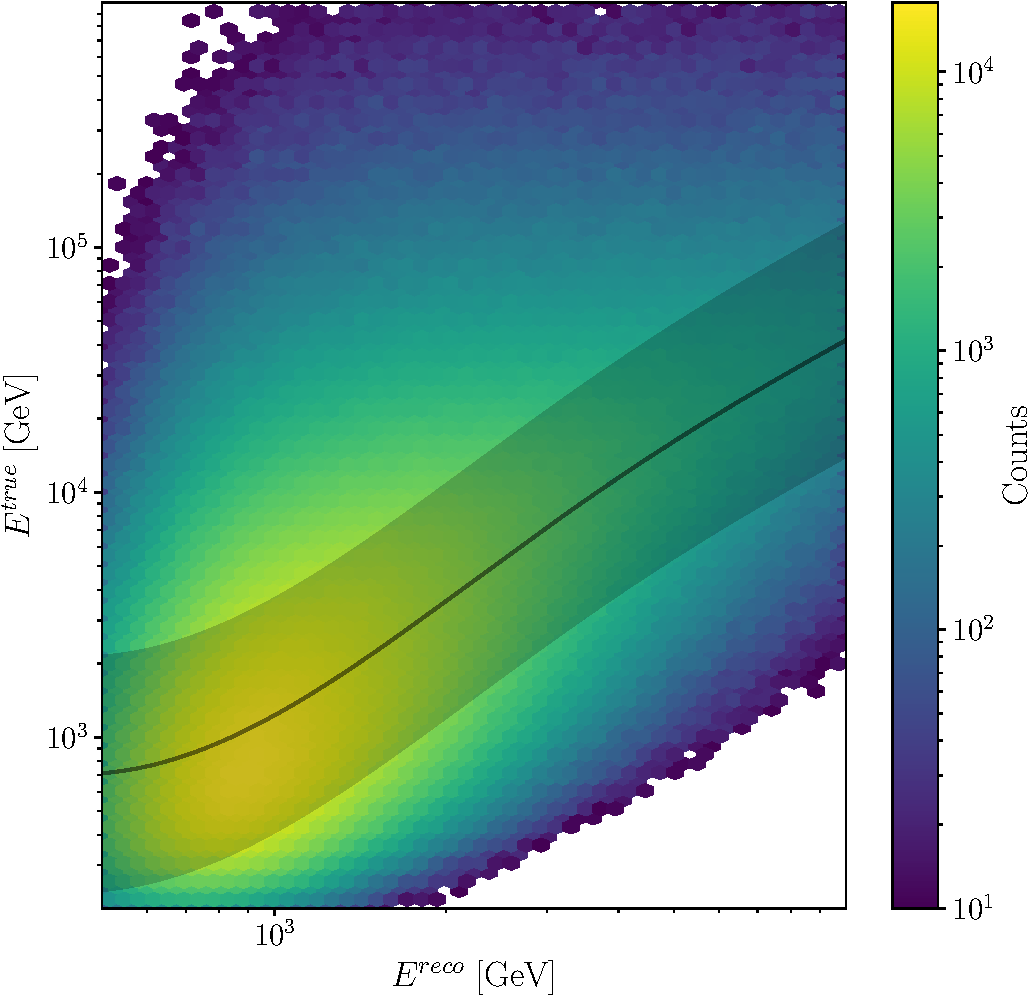
\includegraphics[width=0.4\linewidth]{figures/IC_MC_gpr.pdf} %TODO: another fig here? Aeff?
    \end{center}
    \caption{Relationship between the true and reconstructed muon energy in the IceCube MC sample~\cite{IC2016}}\label{fig:IC_MC_counts}. Shaded area shows the $99.9$th percentile limits predicted by the regressor trained on this set.
 \end{figure}



    



\end{document}